\documentclass[tikz,border=2pt]{standalone}
\usepackage{fontspec}
\setmainfont{texgyreheros}[Extension=.otf,UprightFont=*-regular,BoldFont=*-bold,ItalicFont=*-italic]
\renewcommand{\familydefault}{\rmdefault}
\usepackage{amsmath}
\usetikzlibrary{arrows.meta,calc,positioning}
\begin{document}
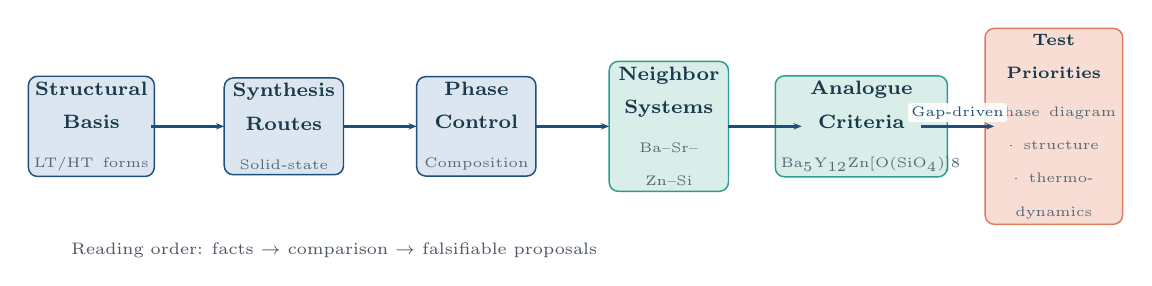
\begin{tikzpicture}[x=1pt,y=1pt, every node/.style={inner sep=0pt}]
\definecolor{nf}{HTML}{DCE6F1}\definecolor{ns}{HTML}{1f4e79}
\definecolor{lc}{HTML}{183A4A}\definecolor{sc}{HTML}{536873}
\node[draw=ns, fill=nf, line width=0.53pt, rounded corners=3.3pt, minimum width=43.1pt, minimum height=29.8pt, text width=41.5pt, align=center, inner sep=2pt, anchor=center] at (28.16pt,117.59pt) {\hyphenpenalty=9000\exhyphenpenalty=9000\relax {\bfseries\fontsize{6.9}{8.1}\selectfont\color{lc}Structural Basis}\\[2.1pt]{\fontsize{5.4}{6.5}\selectfont\color{sc}LT/HT forms}};
\definecolor{nf}{HTML}{DCE6F1}\definecolor{ns}{HTML}{1f4e79}
\definecolor{lc}{HTML}{183A4A}\definecolor{sc}{HTML}{536873}
\node[draw=ns, fill=nf, line width=0.53pt, rounded corners=3.3pt, minimum width=43.1pt, minimum height=29.8pt, text width=38.1pt, align=center, inner sep=2pt, anchor=center] at (97.72pt,117.59pt) {\hyphenpenalty=9000\exhyphenpenalty=9000\relax {\bfseries\fontsize{6.9}{8.1}\selectfont\color{lc}Synthesis Routes}\\[2.1pt]{\fontsize{5.4}{6.5}\selectfont\color{sc}Solid-state}};
\definecolor{nf}{HTML}{DCE6F1}\definecolor{ns}{HTML}{1f4e79}
\definecolor{lc}{HTML}{183A4A}\definecolor{sc}{HTML}{536873}
\node[draw=ns, fill=nf, line width=0.53pt, rounded corners=3.3pt, minimum width=43.1pt, minimum height=29.8pt, text width=38.1pt, align=center, inner sep=2pt, anchor=center] at (167.27pt,117.59pt) {\hyphenpenalty=9000\exhyphenpenalty=9000\relax {\bfseries\fontsize{6.9}{8.1}\selectfont\color{lc}Phase Control}\\[2.1pt]{\fontsize{5.4}{6.5}\selectfont\color{sc}Composition}};
\definecolor{nf}{HTML}{D9EEE9}\definecolor{ns}{HTML}{2a9d8f}
\definecolor{lc}{HTML}{183A4A}\definecolor{sc}{HTML}{536873}
\node[draw=ns, fill=nf, line width=0.53pt, rounded corners=3.3pt, minimum width=43.1pt, minimum height=29.8pt, text width=38.1pt, align=center, inner sep=2pt, anchor=center] at (236.83pt,117.59pt) {\hyphenpenalty=9000\exhyphenpenalty=9000\relax {\bfseries\fontsize{6.9}{8.1}\selectfont\color{lc}Neighbor Systems}\\[2.1pt]{\fontsize{5.4}{6.5}\selectfont\color{sc}Ba--Sr--Zn--Si}};
\definecolor{nf}{HTML}{D9EEE9}\definecolor{ns}{HTML}{2a9d8f}
\definecolor{lc}{HTML}{183A4A}\definecolor{sc}{HTML}{536873}
\node[draw=ns, fill=nf, line width=0.53pt, rounded corners=3.3pt, minimum width=43.1pt, minimum height=29.8pt, text width=58.2pt, align=center, inner sep=2pt, anchor=center] at (306.39pt,117.59pt) {\hyphenpenalty=9000\exhyphenpenalty=9000\relax {\bfseries\fontsize{6.9}{8.1}\selectfont\color{lc}Analogue Criteria}\\[2.1pt]{\fontsize{5.4}{6.5}\selectfont\color{sc}Ba$_{5}$Y$_{12}$Zn[O(SiO$_{4}$)]8}};
\definecolor{nf}{HTML}{F8DDD5}\definecolor{ns}{HTML}{e07a5f}
\definecolor{lc}{HTML}{183A4A}\definecolor{sc}{HTML}{536873}
\node[draw=ns, fill=nf, line width=0.53pt, rounded corners=3.3pt, minimum width=43.1pt, minimum height=29.8pt, text width=45.7pt, align=center, inner sep=2pt, anchor=center] at (375.95pt,117.59pt) {\hyphenpenalty=9000\exhyphenpenalty=9000\relax {\bfseries\fontsize{5.6}{6.6}\selectfont\color{lc}Test Priorities}\\[1.7pt]{\fontsize{4.7}{5.6}\selectfont\color{sc}Phase diagram · structure · thermodynamics}};
\definecolor{ec}{HTML}{1f4e79}
\draw[draw=ec, line width=0.99pt, -{Stealth[length=3.0pt,width=2.3pt]}, rounded corners=2.0pt] (49.69pt,117.59pt) -- (76.18pt,117.59pt);
\definecolor{ec}{HTML}{1f4e79}
\draw[draw=ec, line width=0.99pt, -{Stealth[length=3.0pt,width=2.3pt]}, rounded corners=2.0pt] (119.25pt,117.59pt) -- (145.74pt,117.59pt);
\definecolor{ec}{HTML}{1f4e79}
\draw[draw=ec, line width=0.99pt, -{Stealth[length=3.0pt,width=2.3pt]}, rounded corners=2.0pt] (188.81pt,117.59pt) -- (215.30pt,117.59pt);
\definecolor{ec}{HTML}{1f4e79}
\draw[draw=ec, line width=0.99pt, -{Stealth[length=3.0pt,width=2.3pt]}, rounded corners=2.0pt] (258.37pt,117.59pt) -- (284.86pt,117.59pt);
\definecolor{ec}{HTML}{1f4e79}
\draw[draw=ec, line width=0.99pt, -{Stealth[length=3.0pt,width=2.3pt]}, rounded corners=2.0pt] (327.93pt,117.59pt) -- (354.42pt,117.59pt);
\node[fill=white, fill opacity=0.92, text opacity=1, inner sep=1.2pt, rounded corners=1pt, font=\fontsize{5.0}{5.6}\selectfont, text=ec, anchor=south, align=center] at (341.17pt,118.91pt) {Gap-driven};
\definecolor{tc}{HTML}{4b5563}
\node[anchor=center, font=\fontsize{6.4}{7.7}\selectfont, text=tc] at (115.93pt,72.87pt) {Reading order: facts $\rightarrow$ comparison $\rightarrow$ falsifiable proposals};
\end{tikzpicture}
\end{document}